\section{Discussion}
\label{8.0}
In this section, we provide an in-depth discussion of several critical aspects of our approach. We examine the theoretical necessity of retain data in machine unlearning, present an algorithmic perspective of our BID-LoRA method, and analyze the knowledge leakage phenomenon that motivates our unified framework. These discussions provide deeper insights into the design principles and empirical observations underlying our work.
\vspace{0.0cm}
\subsection{On the Necessity of Retain Buffer in Machine Unlearning}
\label{8.1}
Effective unlearning requires distinguishing what to forget from what to retain. This section investigates whether forget data ($D_f$) or retain buffer ($D_r$, a subset of full retain data $D^\text{full}_r$) can be avoided in classification and face recognition tasks.

We find $D_r$ is fundamentally unavoidable for preserving task-critical knowledge. Without architectural support (e.g., modular pathways), all parameters are adjusted using both $D_f$ and $D^\text{full}_r$ during pretraining, making disentanglement infeasible without $D_r$ access.


\begin{table}[!htbp]
\centering
\caption{Ablation on escape scaling factor $\lambda_{\text{esc}}$. Higher scaling pushes forget embeddings further from retain centroids, improving unlearning}
\begin{tabular}{ccccc}
\toprule
$\lambda_{\text{esc}}$ & $Acc_f \downarrow$ & $Acc_r \uparrow$ & $Acc_n \uparrow$ & $Acc_o \uparrow$ \\
\midrule
0 & 8.80 & 78.57 & 61.07 & 72.74 \\
2 & 4.13 & 80.71 & 63.60 & 75.01 \\
5 & 4.27 & 77.14 & 68.27 & 74.18 \\
\rowcolor{orange!15}
10 & 0.53 & 77.14 & 68.00 & 73.45 \\
\bottomrule
\end{tabular}
\label{tab:escape_ablation}
\end{table}


Only noise-based impair-and-repair methods~\cite{tarun2023fast} and source-free unlearning~\cite{ahmed2025towards} attempt to bypass data dependencies. The former still requires $D_r$. Source-free methods estimate retain data Hessians using only $D_f$ through semi-definite programming, but are limited to convex losses and linear classifiers, making them inapplicable to modern non-convex architectures like transformers and ResNets. In practice, they use frozen pre-trained feature extractors and unlearn only linear heads. While error bounds improve with dimensionality, Hessian storage and inversion become computationally prohibitive.

All established methods for non-convex models critically rely on $D_r$. Weight-importance methods (EWC~\cite{kirkpatrick2017overcoming}, SALUN~\cite{fan2023salun}) compute Fisher information or saliency from $D_r$ to protect retain-relevant weights. SCRUB~\cite{kurmanji2023towards} and GS-LoRA~\cite{zhao2024continual} explicitly leverage $D_r$ to safeguard retained knowledge. CLU methods universally depend on $D_r$: LSF~\cite{shibata2021learning} uses mnemonic codes, UnCLe~\cite{adhikari2025unlearning} employs task embeddings, CLPU-DER++~\cite{liu2022continual} maintains experience replay, and UniCLUN~\cite{chatterjee2024unified} and UG-CLU~\cite{huang2025unified} incorporate $D_r$ for stability.

Generative tasks present exceptions: FLAT~\cite{wang2024llm} solves unlearning without $D_r$ through regularizers, while ESD~\cite{gandikota2023erasing} avoids both $D_f$ and $D_r$ using teacher models to generate synthetic samples.

While $D_f$ can theoretically be avoided through noise-based proxies or source-free methods, no viable approach eliminates $D_r$ dependence for non-convex deep learning without compromising retention performance.

\subsection{Knowledge Leakage Analysis}
\label{8.2}

Can we solve CLU by combining existing CL and MU methods? We pair four combinations (ER-ACE\cite{caccia2021new} + GS\cite{zhao2024continual} ), (DER++ \cite{buzzega2020dark} + FU \cite{tarun2023fast}), (EWC \cite{kirkpatrick2017overcoming} + SalUn\cite{fan2023salun}), and (ER-AML \cite{caccia2021new} + GS\cite{zhao2024continual}) on data-efficient image transformers~\cite{touvron2021training} and FaceTransformer~\cite{zhong2021face} (face recognition). As shown in Fig~\ref{fig:pilot_study}, all exhibit progressive knowledge leakage across CLU cycles, confirming that piecewise solutions fail and a unified framework is necessary.

\begin{figure}[!htbp]
    \centering
    \begin{subfigure}[b]{0.38\linewidth}
        \centering
        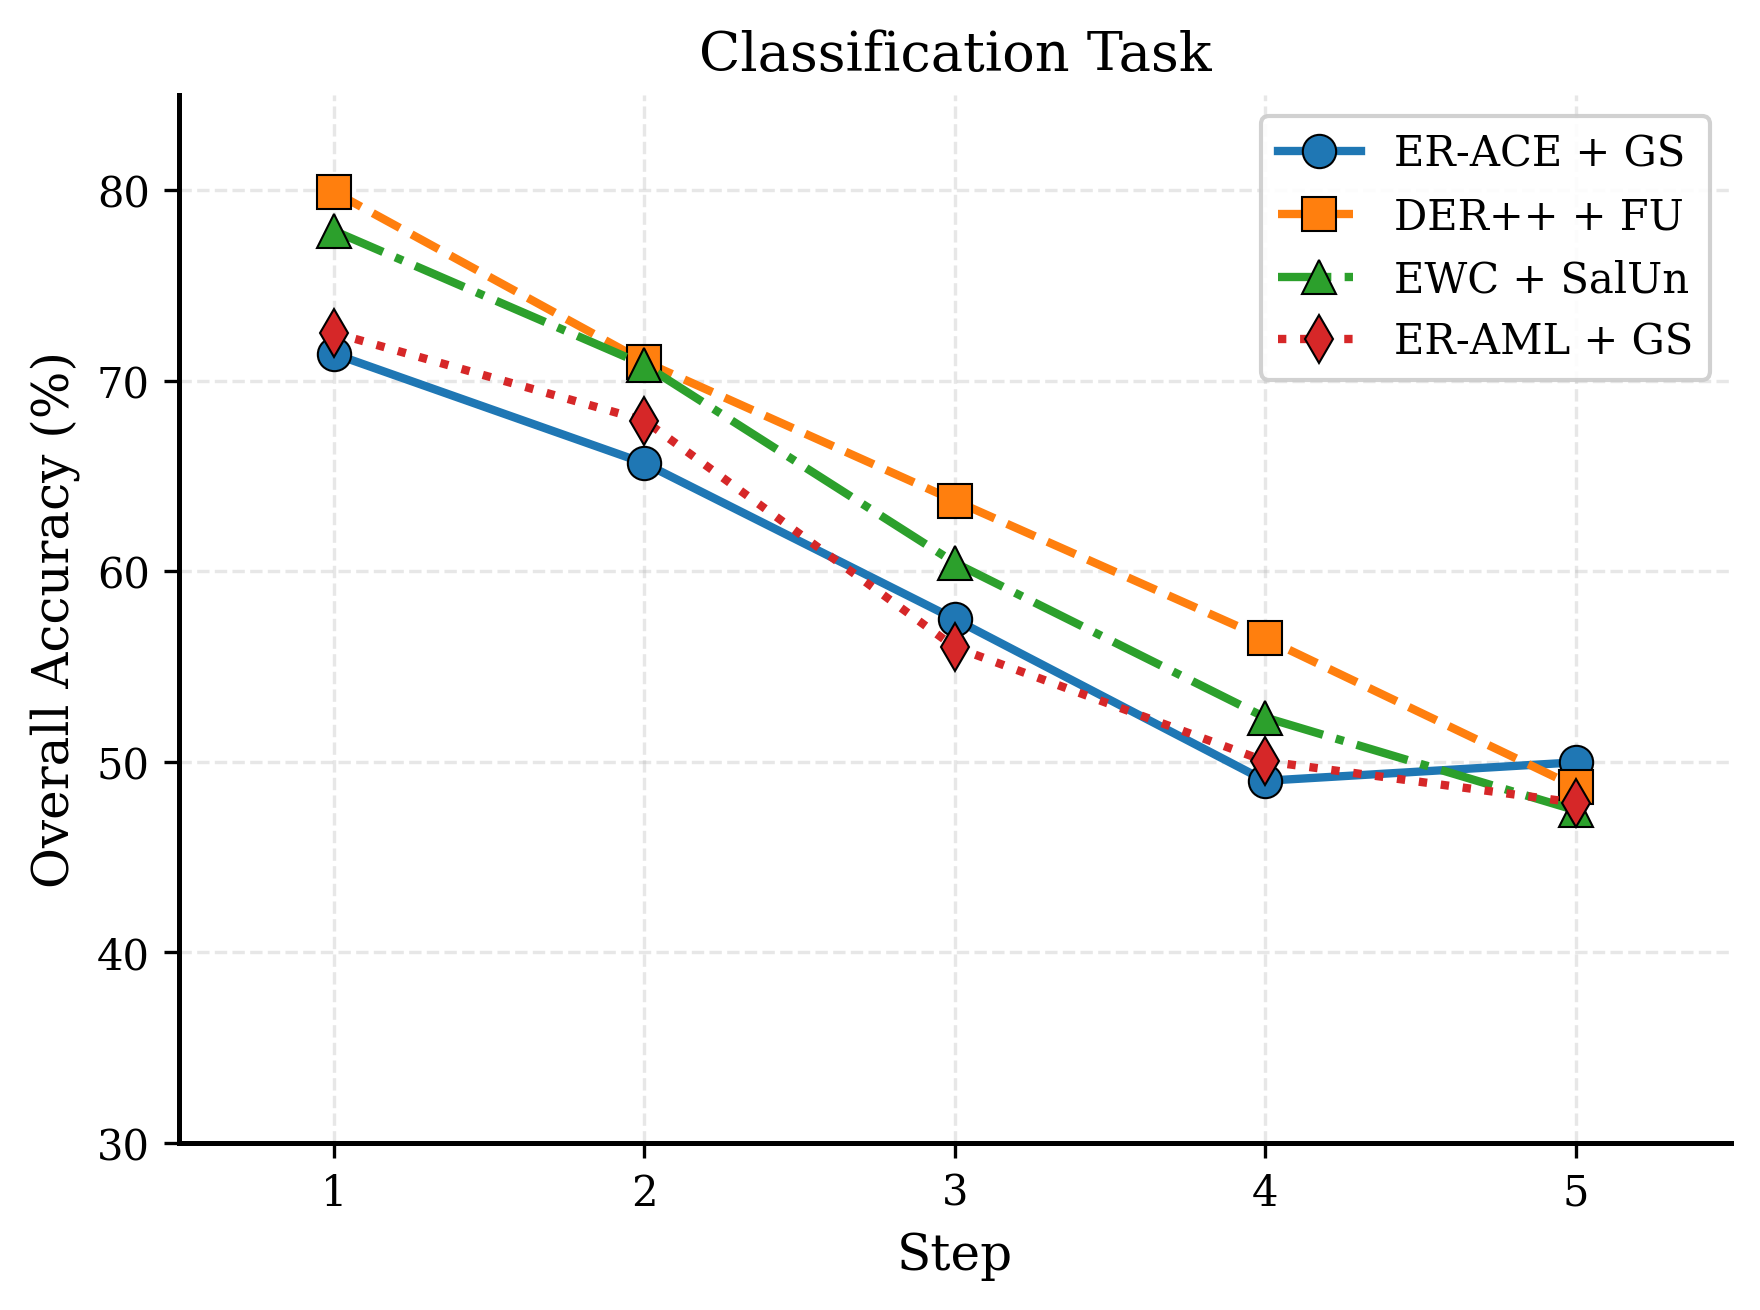
\includegraphics[width=\linewidth]{images/KL_classifaciton.png}
        \caption{CIFAR-100}
    \end{subfigure}
    \hspace{0.5em}
    \begin{subfigure}[b]{0.38\linewidth}
        \centering
        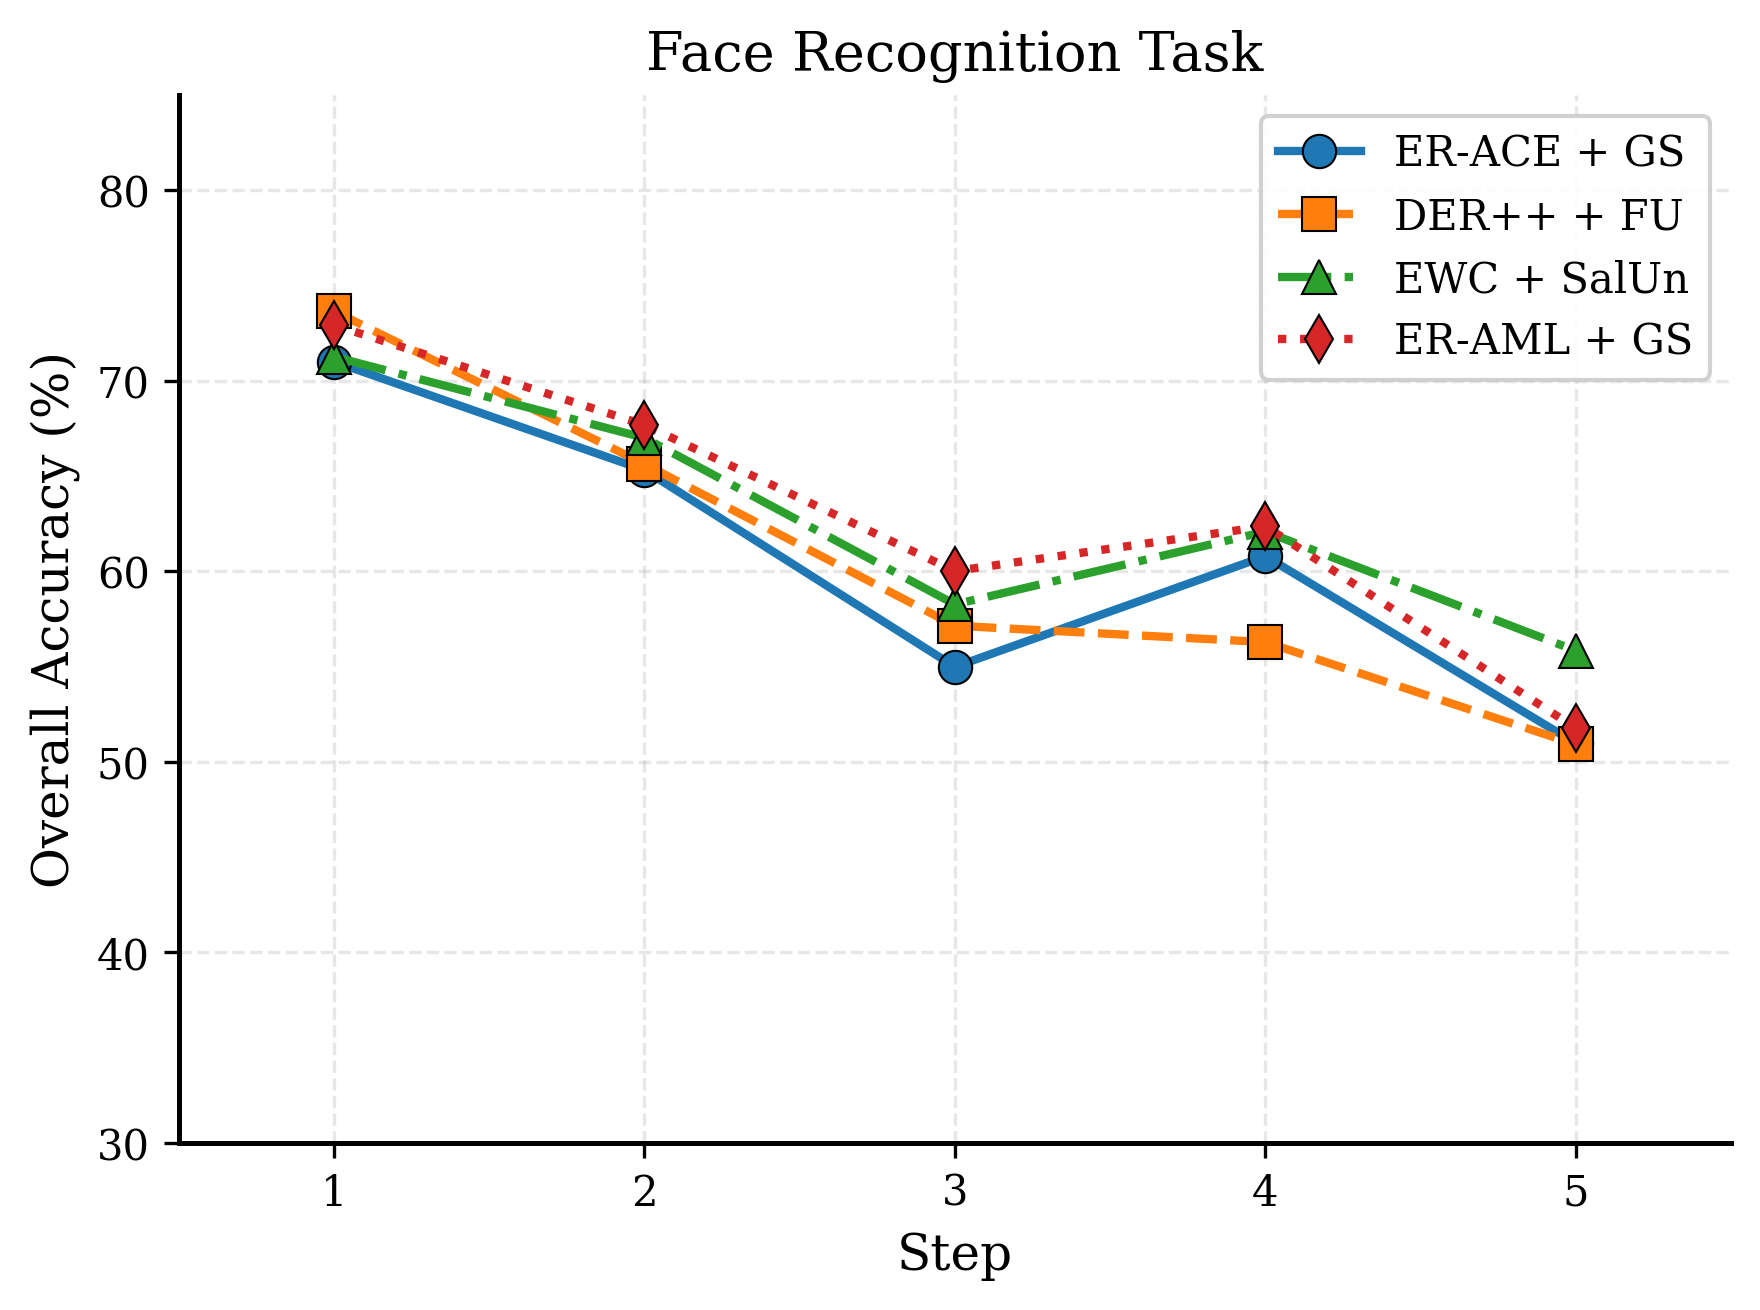
\includegraphics[width=\linewidth]{images/KL_face_Recognition.png}
        \caption{Face Recognition}
    \end{subfigure}
    \caption{Knowledge leakage in CL+MU combinations. Retain accuracy degrades progressively across CLU cycles on both benchmarks.}
    \label{fig:pilot_study}
\end{figure}
